\subsection{Quadtree}
    \begin{itemize}
        \item Faster searching for points within a rectangle
        \item Efficient for querying multiple rectangles
    \end{itemize}
    Data containing two values are inserted into squares. The squares have a maximum number of points they may contain. If a new point would exceed that limit, the square is subdivided into four smaller squares.\\
    {\centering 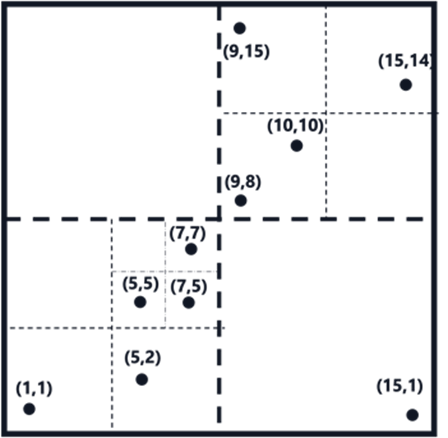
\includegraphics[width = 0.5\linewidth]{src/4_data_structure/images/quadtree.png} \par}

    {\centering\underline{\textbf{Implementation}}\par}
        \lstinputlisting{src/4_data_structure/code/quad_implementation.py}

    {\centering\underline{\textbf{Insert}}\par}
        {\centering 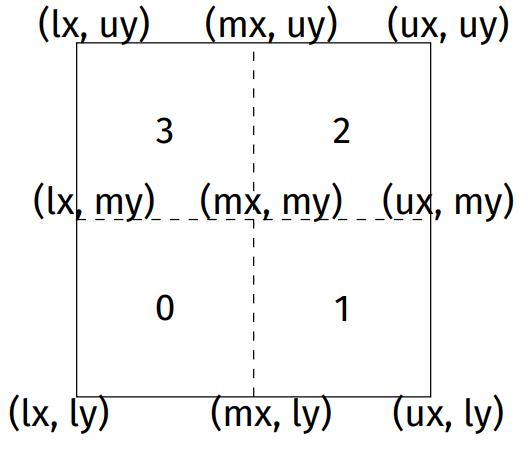
\includegraphics[width = 0.6\linewidth]{src/4_data_structure/images/quad_divide.png} \par}
        \lstinputlisting{src/4_data_structure/code/quad_insert.py}
    
    {\centering\underline{\textbf{Search}}\par}
        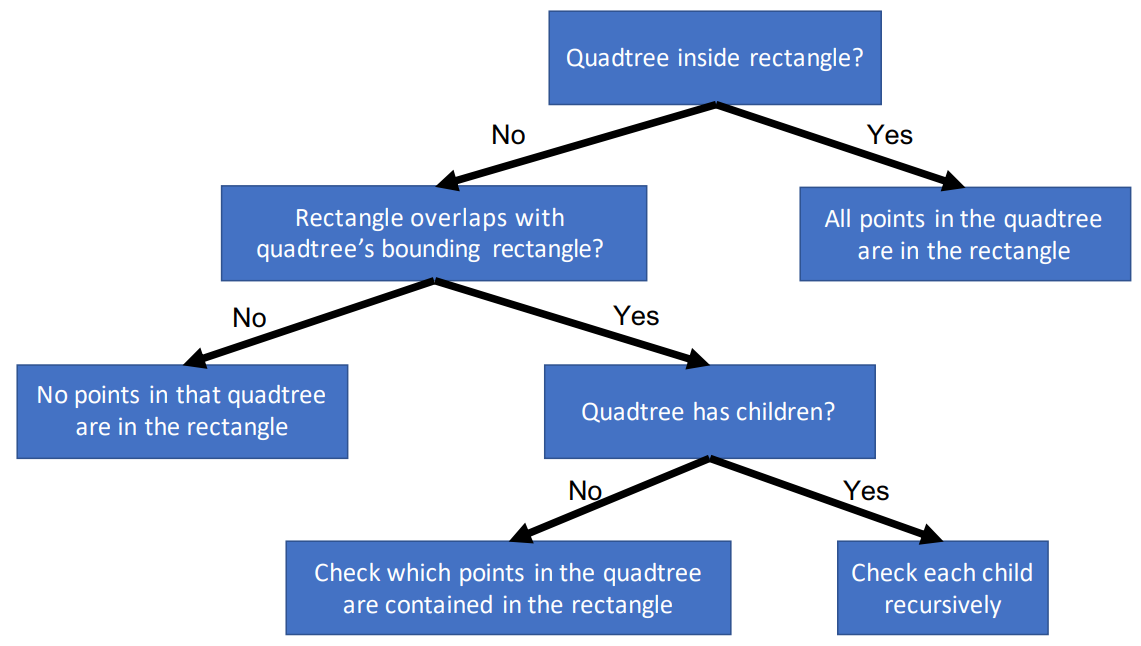
\includegraphics[width = \linewidth]{src/4_data_structure/images/quadtree_rectangle.png}
        \lstinputlisting{src/4_data_structure/code/quad_search.py}
    